\documentclass[a4paper]{article}
\usepackage{cmap}
\usepackage[utf8]{inputenc}
\usepackage[T2A]{fontenc}
\usepackage[english,russian]{babel} 
\usepackage[left=15mm, top=15mm, right=15mm, bottom=30mm, nohead, nofoot]{geometry}
\usepackage{blindtext}  % рыба-текст
\usepackage{graphicx}  % изобржаения
\usepackage{float} % плавающие объекты
\usepackage{wrapfig}  % изобржаения
\usepackage{tikz} % графика
\usepackage{mdframed} % рамки
\usepackage{xcolor} % определение цветов
\usepackage{nicefrac} % красивые дроби
\usepackage{cancel} % сокращение
\usepackage{amsmath,amsfonts,amssymb} % математический пакет
\usepackage{hyperref}  % гиперссылки
\usepackage{fancybox,fancyhdr} % хедер и футер
\usepackage{listings} % код
\usepackage[skip=2pt]{caption} % расстояние между подписью и картинкой
\pagestyle{fancy}
\fancyhf{}
\fancyhead[L]{Лабораторная работа №2}
\fancyhead[R]{\textit{Канонические формы представления динамических систем}}
\fancyfoot[C]{\thepage}
\headsep=4mm
\footskip=13mm
\setlength{\parindent}{0em}
\setlength{\parsep}{0em}
\setlength{\headheight}{12pt}
\setlength{\topmargin}{-38pt}

\definecolor{urlcolor}{HTML}{3454D1}
\definecolor{linkcolor}{HTML}{3454D1}
\hypersetup{
    pdfstartview=FitH,
    linkcolor=linkcolor,
    urlcolor=urlcolor,
    colorlinks=true,
    pdftitle={Лабораторная работа №2},
    pdfauthor={Овчинников П.А.}
}

\definecolor{strings}{rgb}{0,0.6,0}
\definecolor{comments}{rgb}{0,0.3,0}
\definecolor{numbers}{rgb}{0.5,0.5,0.5}
\definecolor{keywords}{rgb}{0.09,0.61,0.95}
\definecolor{background}{rgb}{0.97,0.97,0.97}
\lstdefinestyle{codestyle}{
    backgroundcolor=\color{background},
    commentstyle=\color{comments},
    keywordstyle=\color{keywords},
    stringstyle=\color{strings},
    numberstyle=\tiny\color{numbers},
    basicstyle=\ttfamily\footnotesize,
    breakatwhitespace=false,
    breaklines=true,
    captionpos=b,
    inputencoding=utf8,
    keepspaces=true,
    numbers=left,
    numbersep=5pt,
    showspaces=false,
    showstringspaces=false,
    showtabs=false,
    tabsize=2,
    extendedchars=true,
    literate=
    {а}{{\cyra}}1
    {б}{{\cyrb}}1
    {в}{{\cyrv}}1
    {г}{{\cyrg}}1
    {д}{{\cyrd}}1
    {е}{{\cyre}}1
    {ж}{{\cyrzh}}1
    {з}{{\cyrz}}1
    {и}{{\cyri}}1
    {й}{{\cyrishrt}}1
    {к}{{\cyrk}}1
    {л}{{\cyrl}}1
    {м}{{\cyrm}}1
    {н}{{\cyrn}}1
    {о}{{\cyro}}1
    {п}{{\cyrp}}1
    {р}{{\cyrr}}1
    {с}{{\cyrs}}1
    {т}{{\cyrt}}1
    {у}{{\cyru}}1
    {ф}{{\cyrf}}1
    {х}{{\cyrh}}1
    {ц}{{\cyrc}}1
    {ч}{{\cyrch}}1
    {ш}{{\cyrsh}}1
    {щ}{{\cyrshch}}1
    {ъ}{{\cyrhrdsn}}1
    {ы}{{\cyrery}}1
    {ь}{{\cyrsftsn}}1
    {э}{{\cyrerev}}1
    {ю}{{\cyryu}}1
    {я}{{\cyrya}}1
    {А}{{\CYRA}}1
    {Б}{{\CYRB}}1
    {В}{{\CYRV}}1
    {Г}{{\CYRG}}1
    {Д}{{\CYR96}}1
    {Е}{{\CYRE}}1
    {Ж}{{\CYRZH}}1
    {З}{{\CYRZ}}1
    {И}{{\CYRI}}1
    {Й}{{\CYRISHRT}}1
    {К}{{\CYRK}}1
    {Л}{{\CYRL}}1
    {М}{{\CYRM}}1
    {Н}{{\CYRN}}1
    {О}{{\CYRO}}1
    {П}{{\CYRP}}1
    {Р}{{\CYRR}}1
    {С}{{\CYRS}}1
    {Т}{{\CYRT}}1
    {У}{{\CYRU}}1
    {Ф}{{\CYRF}}1
    {Х}{{\CYRH}}1
    {Ц}{{\CYRC}}1
    {Ч}{{\CYRCH}}1
    {Ш}{{\CYRSH}}1
    {Щ}{{\CYRSHCH}}1
    {Ъ}{{\CYRHRDSN}}1
    {Ы}{{\CYRERY}}1
    {Ь}{{\CYRSFTSN}}1
    {Э}{{\CYREREV}}1
    {Ю}{{\CYRYU}}1
    {Я}{{\CYRYA}}1
}
\lstset{style=codestyle}

\addto\captionsrussian{
  \renewcommand{\contentsname}
    {\centering Содержание}
}
\newcommand{\addsection}[1]{
    \phantomsection
    \addcontentsline{toc}{section}{#1}
    \section*{\centering #1}
}
\newcommand{\addsubsection}[1]{
    \phantomsection
    \addcontentsline{toc}{subsection}{#1}
    \subsection*{\centering #1}
}
\newcommand{\addsubsubsection}[1]{
    \phantomsection
    \addcontentsline{toc}{subsubsection}{#1}
    \subsubsection*{\centering #1}
}

\newmdenv[
    leftmargin = 0.5em,
    skipabove = 0.5em,
    skipbelow = 0.5em,
    linewidth = 1pt,
    rightline = false,
    topline = false,
    bottomline = false
]{quotebox}

\newlength{\tempheight}
\newcommand{\Let}{
\mathbin{\text{\settoheight{\tempheight}{\mathstrut}\raisebox{0.4\pgflinewidth}{
\tikz[baseline=0.5ex,line cap=round,line join=round] \draw (0,0) --++ (0.3em,0) --++ (0,2.3ex) --++ (-0.3em,0);
}}}}
\newcommand*\squared[1]{\tikz[baseline=(char.base)]{
            \node[shape=rectangle,draw,inner sep=4pt] (char) {#1};}}
\newcommand*\msquared[1]{\tikz[baseline=(char.base)]{
            \node[shape=rectangle,draw,inner sep=4pt] (char) {$\displaystyle #1$};}}
\newcommand\argmax[1]{\underset{#1}{\text{argmax}}}
\renewcommand\max[1]{\underset{#1}{\text{max}}}
\newcommand{\at}{\biggr\rvert}
\newcommand{\shiftright}[3]{\makebox[#2][r]{\makebox[#1][l]{#3}}}
\newcommand{\e}{\;\text{e}}
\let\oldint\int
\def\int{\oldint\limits}
\DeclareRobustCommand{\divby}{%
  \mathrel{\vbox{\baselineskip.65ex\lineskiplimit0pt\hbox{.}\hbox{.}\hbox{.}}}%
}

\newcommand\NB{\textbf{N\kern-0.32em\textcolor{red}{B}}}

\begin{document}
\begin{titlepage}
    \begin{center}
    \includegraphics[width=0.18\textwidth]{~/Изображения/itmo_logo.png}\\[10pt]
        Федеральное государственное автономное образовательное \\ учреждение высшего образования \\[6pt]
        САНКТ-ПЕТЕРБУРГСКИЙ НАЦИОНАЛЬНЫЙ \\ ИССЛЕДОВАТЕЛЬСКИЙ УНИВЕРСИТЕТ ИТМО \\[16pt]
        Факультет систем управления и робототехники \vfill
        {\large Лабораторная работа №2} \\[0.5em]
        {\large \textbf{\MakeUppercase{Канонические формы представления динамических систем}}}\\[0.5em]
        Вариант №12
    \end{center}\vfill
    \begin{flushright}
        Студент: Овчинников П.А.\\
        Поток: ЛСАУ R22 бак 4.1.1 \\[0.5em]
        Преподаватели: Лопарев А.В.\\Золотаревич В.П.
    \end{flushright}\vfill
    \begin{center}
        {\small Санкт-Петербург \\ 2024}
    \end{center}
\end{titlepage}
\setcounter{page}{2}
\tableofcontents\newpage
\textbf{Цель работы:} ознакомление с методами взаимного перехода между моделями вход-выход и вход-состояние-выход, а также с каноническими формами представления моделей вход-состояние-выход.
\addsection{Переход от модели вход-выход к модели вход-состояние-выход}
\addsubsection{Порядок выполнения работы}
\begin{itemize}
    \item Построить математические модели вход-состояние-выход в канонической управляемой и канонической наблюдаемой формах в соответствии с вариантом задания. Определить передаточную функцию системы. По варианту задания дано:
    $$n = 2, \quad a_0=0.12, \quad a_1=1, \quad b_0=0.1, \quad b_1=2, \quad b_2=0.$$
    \item Используя блоки \texttt{Transfer Fcn} и \texttt{State-Space} пакета Simulink, осуществить моделирование моделей вход-выход, вход-состояние-выход в канонической управляемой форме и вход-состояние-выход в канонической наблюдаемой форме при ступенчатом единичном входном воздействии и нулевых начальных условиях.
\end{itemize}
% MARK: №1
\addsubsection{Выполнение работы}
Составим знакомое нам дифференциальное уравнение второго порядка:
$$\ddot{y}+\dot{y}+0.12y= 2\dot{u}+0.1u.$$
Запишем его в виде передаточной функции, используя преобразование Лапласа:
$$W(s) = \frac{Y(s)}{U(s)} = \frac{2s+0.1}{s^2+s+0.12}.$$
Такая запись пригодится нам при моделировании системы в Simulink. Теперь найдем канонические формы представления системы.\\[0.5em]
Из дифференциального уравнения, согласно теоретическим сведениям, становится понятно, что каноническая управляемая форма будет иметь следующий вид:
$$A = \begin{vmatrix}
    0 & 1 \\ -0.12 & -1
\end{vmatrix}, \quad B = \begin{vmatrix}
    0 \\ 1
\end{vmatrix}, \quad C^T = \begin{vmatrix}
    0.1 \\ 2
\end{vmatrix}.$$
И в виде системы такая форма записывается так:
$$\begin{cases}
    \dot{x}_1 = x_2, \\ \dot{x_2} = -0.12x_1-x_2+u, \\ y = 0.1x_1+2x_2.
\end{cases}$$
Какноническая наблюдаемая форма же будет иметь такой вид:
$$A = \begin{vmatrix}
    0 & -0.12 \\ 1 & -1
\end{vmatrix}, \quad B = \begin{vmatrix}
    0.1 \\ 2
\end{vmatrix}, \quad C^T = \begin{vmatrix}
    0 \\ 1
\end{vmatrix}.$$
И в виде системы записывается так:
$$\begin{cases}
    \dot{x}_1 = -0.12x_2 + 0.1u, \\ \dot{x}_2 = x_1-x_2+2u, \\ y = x_2.
\end{cases}$$
\newpage
Теперь перейдем к моделированию системы в Simulink с использованием блоков \texttt{Transfer Fcn} и \texttt{State-Space}. Блоку \texttt{КУФ} зададим \texttt{A = [0 1; -0.12 -1]}, \texttt{B = [0; 1]} и \texttt{C = [0.1 2]}, а блоку \texttt{КНФ} зададим \texttt{A = [0 -0.12; 1 -1]}, \texttt{B = [0.1; 2} и \texttt{C = [0 1]}. И вот как будет выглядеть схема:
\begin{figure}[H]
    \centering
    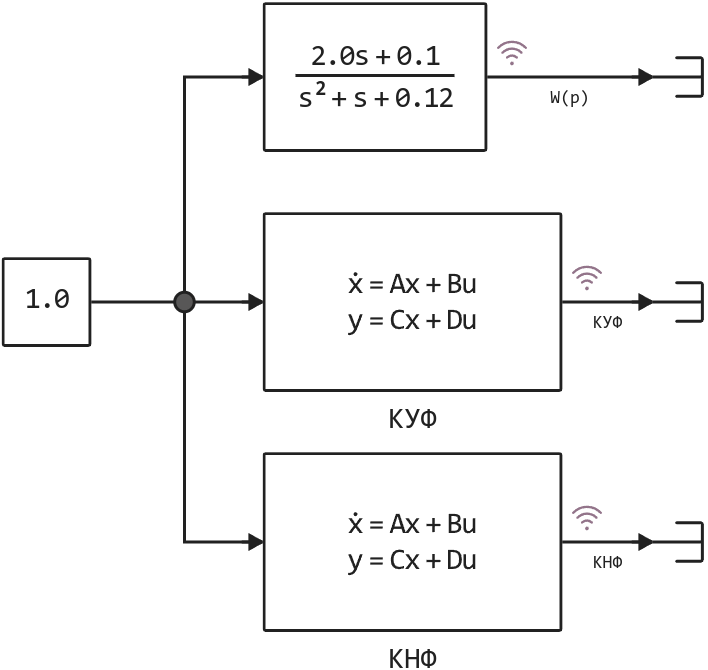
\includegraphics[height=0.23\textheight]{sources/task1_model.png}
    \caption*{Схема моделирования исходной модели вход-выход\\и полученных моделей вход-состояние-выход}
\end{figure}

К отчёту приложён файл \href{run:sources}{\texttt{task1.engee}}, содержащий эту схему, симуляция которой проведена в среде моделирования и симуляции \href{https://start.engee.com/}{Engee}.\\[0.5em]
Приведём графики передаточной функции исходной модели и графики полученных моделей вход-состояние-выход:
\begin{figure}[H]
    \centering
    \begin{minipage}{0.32\textwidth}
        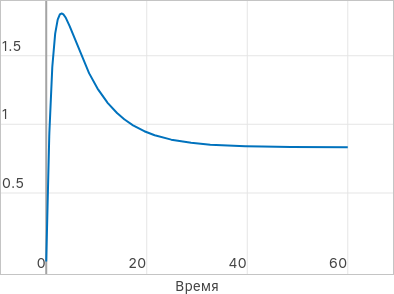
\includegraphics[width=\textwidth]{sources/task1_wp.png}
        \caption*{График $y(t)$ для $W(s)$}
    \end{minipage}
    \hfill
    \begin{minipage}{0.32\textwidth}
        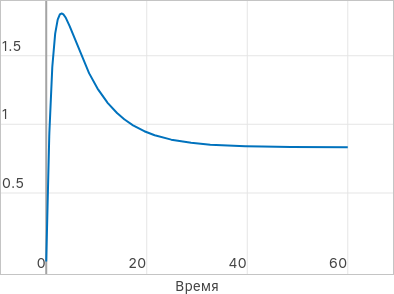
\includegraphics[width=\textwidth]{sources/task1_kuf.png}
        \caption*{График $y(t)$ для КУФ}
    \end{minipage}
    \hfill
    \begin{minipage}{0.32\textwidth}
        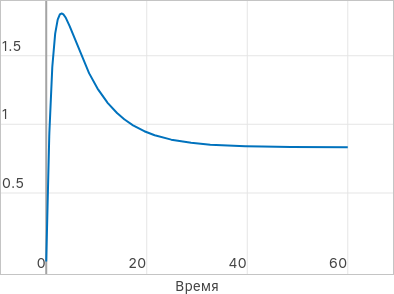
\includegraphics[width=\textwidth]{sources/task1_knf.png}
        \caption*{График $y(t)$ для КНФ}
    \end{minipage}
\end{figure}
Все три графика идентичные, что говорит о том, что нам удалось перейти от модели вход-выход к моделям вход-состояние-выход в канонической управляемой и наблюдаемой формах.



\addsection{Переход от модели вход-состояние-выход к модели вход-выход}
\addsubsection{Порядок выполнения работы}
\begin{itemize}
    \item В соответствии с вариантом задания осуществить расчет передаточной функции системы, а также канонических моделей вход-состояние-выход. По варианту задания дано:
    $$n = 2, \quad A=\begin{vmatrix}
        -1 & 1 \\ -8 & -1
    \end{vmatrix}, \quad B=\begin{vmatrix}
        0.5 \\ 1
    \end{vmatrix}, \quad C^T=\begin{vmatrix}
        5 \\ 1
    \end{vmatrix}.$$
    \item Используя блоки \texttt{Transfer Fcn} и \texttt{State-Space} пакета Simulink, осуществить моделирование исходной модели и полученных моделей вход-выход, вход-состояние-выход в канонической управляемой форме и вход-состояние-выход в канонической наблюдаемой форме, при ступенчатом единичном входном воздействии и нулевых начальных условиях.
    \item Рассчитать матрицы преобразования исходной модели к каноническим формам.
\end{itemize}

% MARK: №2
\addsubsection{Выполнение работы}
Сначала найдем передаточную функцию системы, используя матрицы $A$, $B$ и $C$ и формулу из теоретических сведений:
$$W(s) = C(sI-A)^{-1}B = \begin{vmatrix}
    5 & 1
\end{vmatrix}\left( \begin{vmatrix} s & 0 \\ 0 & s \end{vmatrix} - \begin{vmatrix}
    -1 & 1 \\ -8 & -1
\end{vmatrix}\right)^{-1}\begin{vmatrix}
    0.5 \\ 1
\end{vmatrix} = \begin{vmatrix}
    5 & 1
\end{vmatrix}\begin{vmatrix} s+1 & -1 \\ 8 & s+1 \end{vmatrix}^{-1}\begin{vmatrix}
    0.5 \\ 1
\end{vmatrix} =$$
$$= \begin{vmatrix}
    5 & 1
\end{vmatrix}\begin{vmatrix}
    \frac{s+1}{s^2+2s+9} & \frac{1}{s^2+2s+9} \\
    \frac{-8}{s^2+2s+9} & \frac{s+1}{s^2+2s+9}
    \end{vmatrix}\begin{vmatrix}
    0.5 \\ 1
\end{vmatrix} = \begin{vmatrix}
    \frac{5s-3}{s^2+2s+9} & \frac{s+6}{s^2+2s+9}
    \end{vmatrix}\begin{vmatrix}
        0.5 \\ 1
    \end{vmatrix} = \frac{7s+9}{2s^2+4s+18} = \frac{3.5s+4.5}{s^2+2s+9}.$$
Получаем передаточную функцию системы, из которой можно восстановить модель вход-выход. Теперь найдем канонические формы представления системы. И начнём с канонической управляемой формы, которая имеет вид:
$$A = \begin{vmatrix}
    0 & 1 \\ -9 & -2
\end{vmatrix}, \quad B = \begin{vmatrix}
    0 \\ 1
\end{vmatrix}, \quad C^T = \begin{vmatrix}
    4.5 \\ 3.5
\end{vmatrix}.$$
И в виде системы записывается так:
$$\begin{cases}
    \dot{x}_1 = x_2, \\ \dot{x}_2 = -9x_1-2x_2+u, \\ y = 4.5x_1+3.5x_2.
\end{cases}$$
Теперь найдем каноническую наблюдаемую форму, которая имеет вид:
$$A = \begin{vmatrix}
    0 & -9 \\ 1 & -2
\end{vmatrix}, \quad B = \begin{vmatrix}
    4.5 \\ 3.5
\end{vmatrix}, \quad C^T = \begin{vmatrix}
    0 \\ 1
\end{vmatrix}.$$
И в виде системы записывается так:
$$\begin{cases}
    \dot{x}_1 = -9x_2+4.5u, \\ \dot{x}_2 = x_1-2x_2+3.5u, \\ y = x_2.
\end{cases}$$
Схема моделирования системы в Simulink идентична той, что была выше:
\begin{figure}[H]
    \centering
    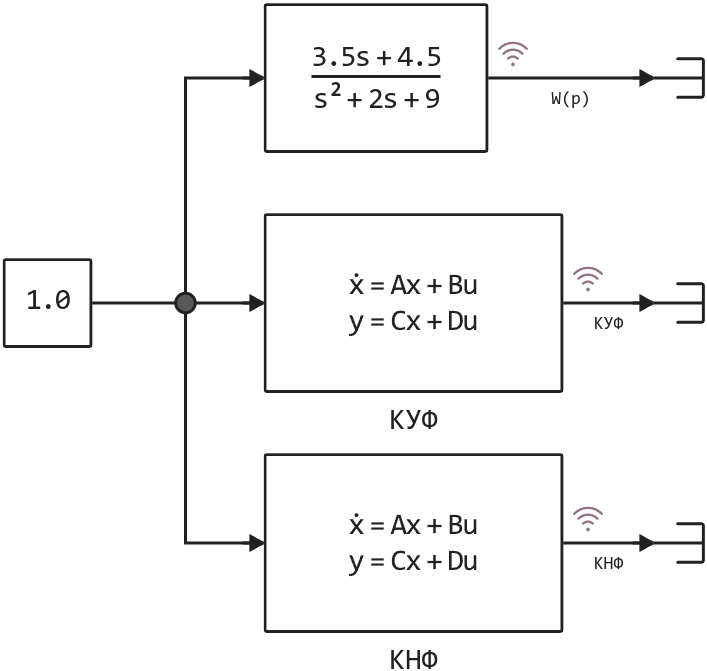
\includegraphics[height=0.23\textheight]{sources/task2_model.png}
    \caption*{Схема моделирования исходной модели вход-состояние-выход\\и полученных моделей вход-выход}
\end{figure}
К отчёту так же приложён файл \href{run:sources}{\texttt{task2.engee}}, содержащий эту схему, симуляция которой проведена в среде моделирования и симуляции \href{https://start.engee.com/}{Engee}.\newpage
Приведём графики передаточной функции исходной модели и графики полученных моделей вход-состояние-выход:
\begin{figure}[H]
    \centering
    \begin{minipage}{0.32\textwidth}
        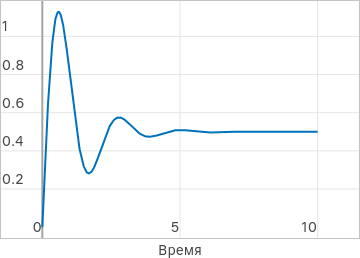
\includegraphics[width=\textwidth]{sources/task2_wp.png}
        \caption*{График $y(t)$ для $W(s)$}
    \end{minipage}
    \hfill
    \begin{minipage}{0.32\textwidth}
        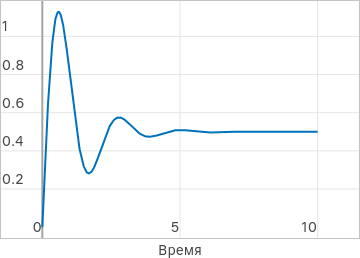
\includegraphics[width=\textwidth]{sources/task2_kuf.png}
        \caption*{График $y(t)$ для КУФ}
    \end{minipage}
    \hfill
    \begin{minipage}{0.32\textwidth}
        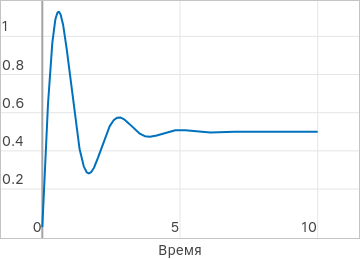
\includegraphics[width=\textwidth]{sources/task2_knf.png}
        \caption*{График $y(t)$ для КНФ}
    \end{minipage}
\end{figure}
И вновь они идентичны --- нам удалось перейти от модели вход-состояние-выход к модели вход-выход.



\addsection{Замена базиса в пространстве состояний}
\addsubsection{Порядок выполнения работы}
\begin{itemize}
    \item В соответствии с вариантом матрицы преобразования координат, построить модель, подобную модели из предыдущего задания. По варианту задания дано:
    $$M=\begin{vmatrix}
        5 & 0 \\ 5 & 1
    \end{vmatrix}$$
    \item Используя блоки \texttt{State-Space}, осуществить моделирование исходной и преобразованной систем при ступенчатом единичном входном воздействии и нулевых начальных условиях. На экран вывести выходные переменные двух систем.
\end{itemize}
% MARK: №3
\addsubsection{Выполнение работы}
Выполним замену базиса в пространстве состояний, пользуясь тем, что матрицы подобных модолей связаны матрицей преобразования координат следующим образом:
$$A' = M^{-1}AM, \quad B' = M^{-1}B, \quad C' = CM.$$
Произведём расчёты, чтобы найти матрицы $A'$, $B'$ и $C'$:
$$M^{-1} = \begin{vmatrix}
    5 & 0 \\ 5 & 1
\end{vmatrix}^{-1} = \begin{vmatrix}
    0.2 & 0 \\ -1 & 1
\end{vmatrix}$$
$$M^{-1}AM = \begin{vmatrix}
    0.2 & 0 \\ -1 & 1
\end{vmatrix}\begin{vmatrix}
    -1 & 1 \\ -8 & -1
\end{vmatrix}\begin{vmatrix}
    5 & 0 \\ 5 & 1
\end{vmatrix} = \begin{vmatrix}
    -0.2 & 0.2 \\ -7 & -2
\end{vmatrix}\begin{vmatrix}
    5 & 0 \\ 5 & 1
\end{vmatrix} = 
\begin{vmatrix}
    0 & 0.2 \\ -45 & -2
\end{vmatrix}$$
$$M^{-1}B = \begin{vmatrix}
    0.2 & 0 \\ -1 & 1
\end{vmatrix}\begin{vmatrix}
    0.5 \\ 1
\end{vmatrix} = \begin{vmatrix}
    0.1 \\ 0.5
\end{vmatrix}$$
$$CM = \begin{vmatrix}
    5 & 1
\end{vmatrix}\begin{vmatrix}
    5 & 0 \\ 5 & 1
\end{vmatrix} = \begin{vmatrix}
    30 & 1
\end{vmatrix}$$\newpage
Построим схему моделирования системы в Simulink, используя блоки \texttt{State-Space} и задав матрицы $A'$, $B'$ и $C'$ на втором блоке:
\begin{figure}[H]
    \centering
    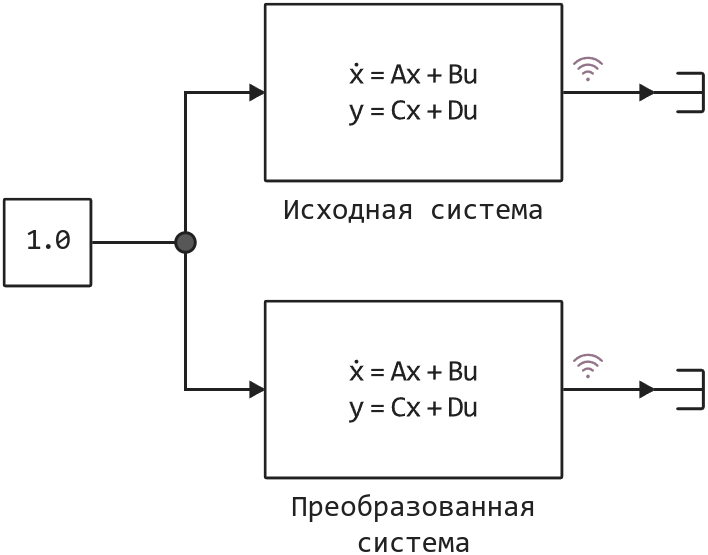
\includegraphics[height=0.23\textheight]{sources/task3_model.png}
    \caption*{Схема моделирования исходной и преобразованной систем}
\end{figure}
К отчёту приложён файл \href{run:sources}{\texttt{task3.engee}}, содержащий эту схему. Симуляция проведена в среде моделирования и симуляции \href{https://start.engee.com/}{Engee}.\\[0.5em]
И выведем графики исходной и преобразованной систем:
\begin{figure}[H]
    \centering
    \begin{minipage}{0.4\textwidth}
        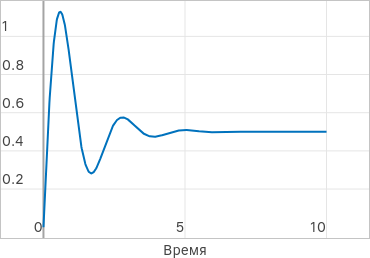
\includegraphics[width=\textwidth]{sources/task3_original.png}
        \caption*{График $y(t)$ для исходной системы}
    \end{minipage}
    \hspace{2em}
    \begin{minipage}{0.4\textwidth}
        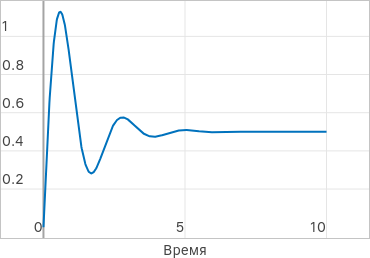
\includegraphics[width=\textwidth]{sources/task3_modified.png}
        \caption*{График $y(t)$ для преобразованной системы}
    \end{minipage}
\end{figure}

\addsection{Выводы}
В ходе выполнения лабораторной работы мы изучили методы взаимного перехода между моделями вход-выход и вход-состояние-выход, а также канонические формы представления моделей вход-состояние-выход. Мы научились строить математические модели вход-состояние-выход в канонической управляемой и наблюдаемой формах, а также осуществлять моделирование этих моделей в среде моделирования. Также мы научились заменять базис в пространстве состояний и строить модели преобразованных систем.

\end{document}